\section{Missent Letters}



\begin{figure}[htp]
\centering
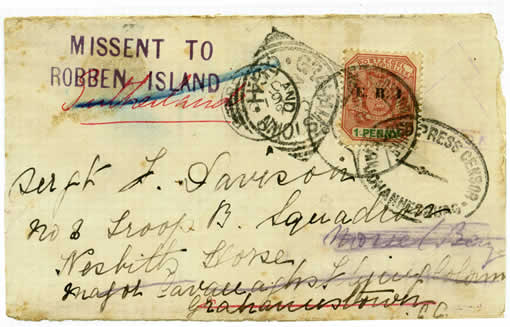
\includegraphics[width=.80\textwidth]{../cape-of-good-hope/missent-letters/Missent-Robben-Island-Front.jpg}
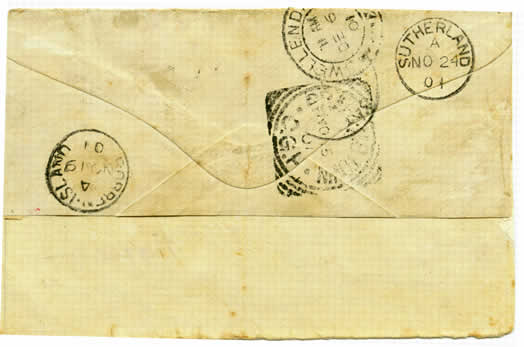
\includegraphics[width=.80\textwidth]{../cape-of-good-hope/missent-letters/1.jpg}
\caption{Cover with SP 5, the explanatory mark 
'Missent to Robben Island'; in November 1901. Note the 
Johannesburg press censor's marking in use during the Anglo-Boer War. 
The cover was sorted into the wrong mailbag.
}
\end{figure}


Often due to errors made by mail sorters, letters were forwarded to 
incorrect destinations. Special handstamps (Goldblatt  SP 1 to 5) 
were used to identify this missent mail. Missent mail was also marked in manuscript. 
Two were in use in Cape Town G.P.O (SP 1 and SP 2). Port Elizabeth, Paarl, 
Robben Island, Grahamstown and Kimberley hd their own official handstamp 
for this purpose.  The country postmasters were not provided with 
handstamps but made a manuscript note on the letter which they 
initialed, e.g. 'Missent to Paarl'.

The Postmaster of Willomore used an improvised combination of 
marking the word 'missent'in manuscript and a locally made stamp 
with the name 'Willomore' to mark 'missent mail'. 
See an example here. See also examples of manuscript markings 
as used at Sea-Point here.

An interesting cover was described in the London Philatelist by Alan Drysdall<sup>1</sup> and 
shown in the figure below. It bears the Cape of Good Hope, Cape Town Missent marking.
\begin{figure}[htp]
\centering
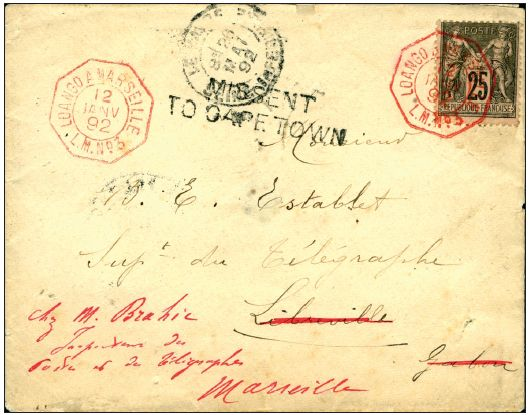
\includegraphics[width=.95\textwidth]{../cape-of-good-hope/MISSENT-LETTERS/missent-cape-town.jpg}
\caption{Cover from France to Marsielle via Libreville and Cape Town. The cover 
was described by Alan Drysdall in the London Philatelist and the Illustration was credited to
John and Mark Taylor.
}
\end{figure}

1. Drysdall A, \textit{Missent to Cape Town}, London Philatelist, December 2008, 117-400. (LP1361.pdf)
                                           